\documentclass[crop={true},border={0.2cm}]{standalone}

\usepackage{hyperref}
\usepackage{pxfonts}
\usepackage{tikz}
\usepackage{xargs}

\usetikzlibrary{arrows.meta}
\usetikzlibrary{decorations.markings}
\usetikzlibrary{decorations.pathmorphing}
\usetikzlibrary{decorations.text}
\usetikzlibrary{shapes}
\usetikzlibrary{shapes.geometric}
\usetikzlibrary{shapes.multipart}

\hypersetup{pdftex,pdflang={en-GB},colorlinks={true},bookmarks={false},urlcolor={red}}
\newcommandx{\CIRCLED}[1]{\tikz[baseline=(char.base)]{\node[shape=circle,draw,inner sep=2pt] (char) {#1};}}
\newlength{\SEP}\setlength{\SEP}{0.2cm}

% =============================================================================

\begin{document}
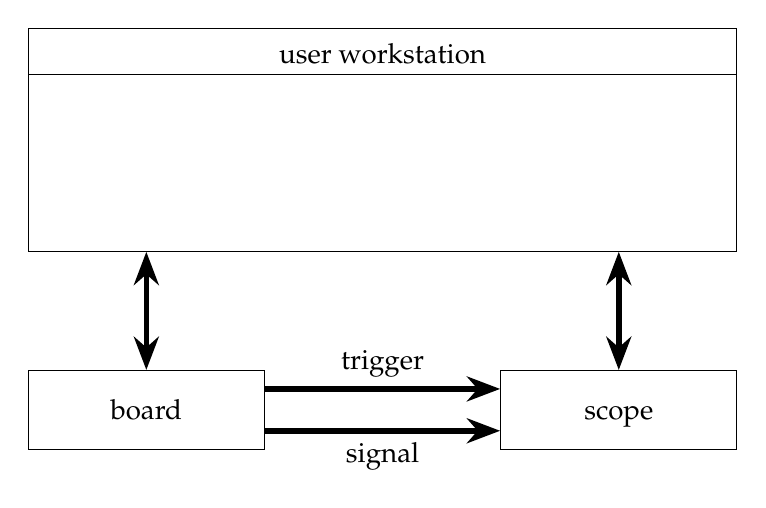
\begin{tikzpicture}

\tikzstyle{component}=[rectangle split,rectangle split parts={2},rectangle split ignore empty parts={false},rectangle split empty part height={2.0cm},minimum width={9.0cm},text height={2.0ex},align={center}]
\tikzstyle{network}=[cloud,cloud ignores aspect,minimum width={8.0cm},minimum height={5.5cm}]

% components: nodes

\node [draw,anchor={south},component] (C2) {\nodepart{text} user workstation} ;

% components: board and scope

\node at ([shift={(+0.0cm,-1.5cm)}] C2.south west) [draw,rectangle,anchor={north west},minimum width={3.0cm},minimum height={1.0cm}] (B) {\raisebox{-0.0em}{board}} ;
\node at ([shift={(+0.0cm,-1.5cm)}] C2.south east) [draw,rectangle,anchor={north east},minimum width={3.0cm},minimum height={1.0cm}] (S) {\raisebox{-1.0em}{scope}} ;

% connections: board and scope

\draw [{ Stealth[open]-Stealth[open]},line width={2pt}] (B.north) -- (B.north |- C2.south) ;
\draw [{ Stealth[open]-Stealth[open]},line width={2pt}] (S.north) -- (S.north |- C2.south) ;

\draw [{-Stealth[open]},line width={2pt}] (B.10)  -- node [midway,above] {trigger} (B.10  -| S.west) ;
\draw [{-Stealth[open]},line width={2pt}] (B.350) -- node [midway,below] {signal}  (B.350 -| S.west) ;

\end{tikzpicture}
\end{document}

% =============================================================================
